%Set document class
\documentclass{article}

%Load math symbol packages
\usepackage{amsmath}
\usepackage{amssymb}
\usepackage{tikz} 
\usepackage{hyperref}
\usepackage{mathtools}
\usepackage{indentfirst}
\usepackage{graphicx}

%User defined commands
\newcommand{\var}{\operatorname{Var}}

\begin{document}
\begin{center}
	\huge{\bf Math 181A: Homework 1} \\
	Merrick Qiu 
\end{center}

\subsection*{Problem 1: 3.6.6}
The expectation of $Y$ is 
\begin{align*}
	E[Y] &= \int_0^k \frac{2y^2}{k^2} \,dy \\
	&= \left[\frac{2y^3}{3k^2}\right]_0^k \\
	&= \frac{2}{3}k.
\end{align*}

The expectation of $Y^2$ is 
\begin{align*}
	E[Y^2] &= \int_0^k \frac{2y^3}{k^2} \,dy \\
	&= \left[\frac{y^4}{2k^2}\right]_0^k \\
	&= \frac{1}{2}k^2.
\end{align*}

Thus 
\begin{align*}
	\var(Y) &= E[Y^2] - E[Y]^2 \\
	&= \frac{1}{2}k^2 - \frac{4}{9}k^2 \\
	&= \frac{k^2}{18} \\
	&= 2.
\end{align*}

and so $k = 6$.
\newpage



\subsection*{Problem 2: 3.9.20}
Expectation is linear so 
\begin{align*}
	E[W] &= E[4X+6Y] \\
	&= 4E[X] + 6E[Y] \\
	&= 4np_x + 6mp_y.
\end{align*}

Using the properties of variance yields
\begin{align*}
	\var(W) &= \var(4X+6Y) \\
	&= 16\var(X) + 36\var(Y) \\
	&= 16np_x(1-p_x) + 36mp_y(1-p_y).
\end{align*}
\newpage 

\subsection*{Problem 3: 4.3.33}

Using a Z-table, we have that
\begin{align*}
	P(\overline{Y} > 103) 
	&= P(\frac{\overline{Y} - 100}{16} > \frac{3}{16}) \\
	&\approx P(Z > 0.56) \\
	&\approx 0.29
\end{align*}

Using a Z-table, we have that for a single variable
\begin{align*}
	P(Y > 103) 
	&= P(\frac{Y-100}{16/\sqrt{9}} > \frac{3}{16/\sqrt{9}}) \\
	&\approx P(Z > 0.19) \\
	&\approx 0.42
\end{align*}

From the PMF of the binomial distribution,
the probability that exact 3 of the IQs is above 103 is 
$\binom{9}{3}(0.42)^3(1-0.42)^6 \approx 0.24$.
\newpage 

\subsection*{Problem 4: 4.3.34}
Using the weak law of large numbers,
\begin{align*}
	P(1.9 \leq \overline{Y} \leq 2.1) \geq 0.99
	&\implies P(\frac{1.9}{2/\sqrt{n}} \leq \overline{Y} \leq \frac{2.1}{2/\sqrt{n}}) \geq 0.99  = P(-2.58 \leq Z \leq 2.58)\\
	&\implies  2.58 \leq \frac{0.1}{2/\sqrt{n}}\\
	&\implies n \geq 2663.
\end{align*}
\newpage 

\subsection*{Problem 5: Prove Weak Law of Large Numbers}
Let $\overline{X_n}$ be the mean of $n$ i.i.d random variables, $X_1,\hdots,X_n$.
Let $\mu$ be the mean and let $\sigma^2$ be the variance of each i.i.d variable.
Let $\epsilon > 0$.
Applying Chebyshev's inequality to $\overline{X}$ yields 
\begin{align*}
	\lim_{n \to \infty} P(|\overline{X_n} - \mu| \geq \epsilon) 
	&\leq \lim_{n \to \infty} \frac{\var{\overline{X_n}}}{\epsilon^2} \\
	&= \lim_{n \to \infty} \frac{\sigma^2}{n\epsilon^2} \\
	&= 0.
\end{align*}

Since probability cannot be negative, this implies that 
\[
	\lim_{n \to \infty} P(|\overline{X_n} - \mu| \geq \epsilon) = 0.
\]
\newpage 

\subsection*{R simulation}
The paths representing the means of the random variables 
appear to converge to the mean of 1, shown by the red line.
This agrees with the Law of Large Numbers, which says that
as n grows, the mean will approach the average of the distribution.

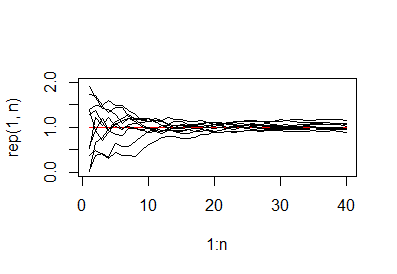
\includegraphics{hw1part1.png} 

Again the paths converge to the mean of  
$E[X^2] = \int_0^2 \frac{1}{2}x^2 = \frac{4}{3}$.

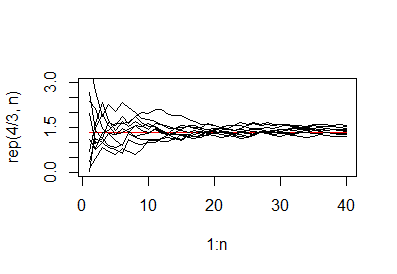
\includegraphics{hw1part2.png}

\end{document}

